\documentclass[12pt]{article}
\usepackage[margin=1.5cm]{geometry}
\usepackage{parskip}
\usepackage{amsmath}
\usepackage{amssymb}
\usepackage{amsfonts}
\usepackage{enumitem}
\usepackage{graphicx}
\usepackage{stmaryrd}
\graphicspath{ {./images/} }


\begin{document}
\begin{enumerate}[label=(\alph*)]

  \item
    A register inference graph is constructed through live variable analysis.

    On a portion of code, we run live variable analysis which tells us which variables are live at each point in a program. If two variables are simultaneously live, we know that they cannot be allocated to the same register. Therefore, we build a clash graph by creating a node for each variable, and joining two variables if they are simultaneously live.

    This graph can be used for register allocation, since the problem of register allocation becomes producing a colouring for the clash graph, since simultaneously live nodes will never be assigned the same colour (i.e. register).

    \item

      We annotate the code with LVA sets:

\begin{verbatim}
L0   MOV p, r0            {t6, r0}
L1   MOV i, #0            {p, t6}
L2   CMP p, #0; BEQ L10   {i, p, t6}
L3:  MOV t3, i            {i, t6}
L4   ADD t4, t3, #1       {t3}
L5   MOV i, t4            {t4}
L6   MOV t5, p            {i, p}
L7   LDR t6, [t5, #4]     {i, t5}
L8   MOV p, t6            {i, t6}
L9   CMP t6, #0; BNE L3   {i, t6}
L10: MOV r0, i            {i}
L11  RET                  {r0}
\end{verbatim}

This produces the following clash graph:

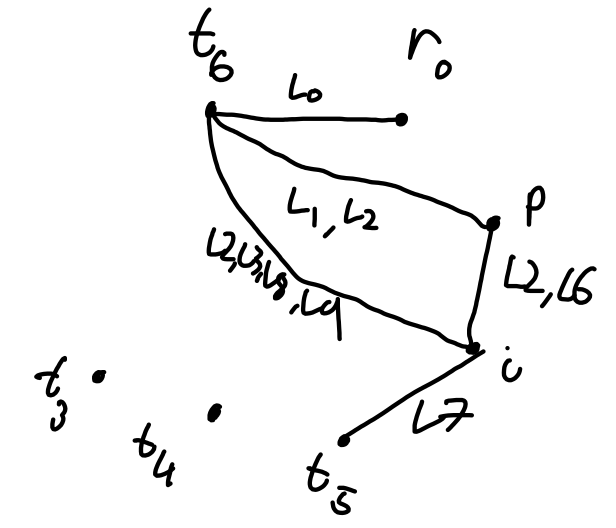
\includegraphics[scale=0.3]{clashgraph}

\item
  By putting a program into SSA form, we minimise the live ranges of all of its variables. By putting a program into an SSA form, a variable will become live after its definition, and then stop being live at its final use. When the program is not in SSA form, this will still be true, but we might have later points in the program where the variable is redefined and used again, making that variable clash with other variables, whereas in SSA form we would be using a different variable entirely.

  In SSA form, live ranges remain the same as they were before, but two non-contiguous ranges are never for the same variable. Therefore, we can say with certainty that the clash graph produced on a piece of SSA form code will have nodes with smaller or equal degree than the corresponding non-SSA form code.

  In fact, we could even view each node in our clash graph as being split into many separate nodes, for each of its SSA-created variants, and each of these must have degree less than or equal to the original node.

  Therefore, we expect $l \leq k$, for all programs.
        
    \end{enumerate}
\end{document}
